\documentclass[11pt]{article}

\usepackage[margin=1in]{geometry}
\usepackage{amsmath}
\usepackage{booktabs}
\usepackage{graphicx}
\usepackage{hyperref}
\usepackage[numbers,sort&compress]{natbib}
\usepackage{caption}
\usepackage{subcaption}
\usepackage{xcolor}

\graphicspath{{figures/}}

\title{Design of Experiments for Sparse Autoencoder Feature Stability: A Worked Gemma Scope Case Study}
\author{Larry Richards\\\href{mailto:papers@source1.jp}{papers@source1.jp}}
\date{\today}

\begin{document}
\maketitle

\begin{abstract}
Sparse autoencoders (SAEs) offer a practical way to transform transformer residual-stream activations into sparse feature vectors, but it is not yet clear how stable those feature vectors are under controlled prompt perturbations. This report frames SAE activations as response variables in a classical Design of Experiments (DoE) setting. The goal is methodological: to show what becomes visible when mechanistic-interpretability measurements are collected under a fully crossed factorial design rather than an ad hoc prompt sweep. We study Gemma Scope residual-stream SAEs on Gemma-2-2B-Instruct using 405 unique prompts crossing content domain, role framing, surface paraphrase, and language register; each prompt is measured at three transformer layers, yielding 1215 prompt-by-layer cells. We persist raw residual activations and sparse SAE encodings, then analyze four scalar response variables: activation norm, number of nonzero SAE features, top-1 SAE activation magnitude, and feature entropy. Five-factor ANOVA shows that layer is the dominant source of variance across all responses, with partial $\eta^2$ between 0.907 and 0.993. Crucially, the design also exposes interaction structure: two-way interactions with layer, especially content-domain-by-layer and role-framing-by-layer, are large. A focused permutation test on a 27-cell layer-12 similarity matrix finds role-framing block structure (observed within-minus-between similarity 0.0912, 0/1000 null draws greater than or equal to observed), while paraphrase and register do not show comparable block structure. A retrospective categorical Latin-style subsample with 27 prompt cells recovers the full-factorial main-effect ranking well across the four response variables, but smaller subsamples degrade sharply. The experiment demonstrates that factorial measurement reveals interaction structure invisible to single-factor prompt sweeps, including substantial layer-by-content and layer-by-role-framing interactions that reorder the apparent importance of prompt factors at different depths.
\end{abstract}

\section{Introduction}

Sparse autoencoders have become a central tool in recent mechanistic interpretability work because they can decompose dense model activations into overcomplete sparse feature dictionaries. The resulting coordinates are not guaranteed to be semantic, causal, or stable, but they are much more directly inspectable than raw residual-stream vectors. This experiment asks a narrower measurement question: under a controlled factorial prompt design, how much do SAE-derived feature patterns move when the prompt content, role framing, paraphrase, register, and layer are varied?

The motivation is practical and methodological. If SAE features are to be used as dependent variables in downstream experiments, then experimental designs need to know which perturbations dominate the measured feature geometry. A prompt factor that changes ordinary text while leaving feature geometry nearly invariant can be treated differently from a factor that strongly reorganizes feature activations. Conversely, if layer dominates every response, then single-layer conclusions should be framed as layer-local rather than model-global.

A central point of this report is that SAE activations can be treated as response variables in a designed experiment. Without a crossed design, prompt comparisons can reveal that feature activations change, but they cannot cleanly attribute that change to content, role framing, paraphrase, register, layer, or their interactions. The factorial design used here makes interaction structure visible. Several of the largest effects are not simple prompt-side main effects, but interactions between layer and content or layer and role framing. This is precisely the kind of structure that ad hoc prompt sweeps are poorly equipped to detect.

The present experiment uses Gemma-2-2B-Instruct and Gemma Scope residual-stream SAEs. It is deliberately small but fully crossed: three content domains, three role framings, three surface paraphrase conditions, three language-register conditions, five content IDs per domain, and three layers. The core contribution of this report is not a semantic interpretation of any SAE feature. Instead, it is a measurement scaffold: a persisted dataset of SAE encodings, a set of response variables, a five-factor ANOVA decomposition, a retrospective sampling comparison, and a quantitative test of block structure in feature space.

\paragraph{Methodological contribution.}
The worked example demonstrates what the discipline of DoE and factorial analysis adds to mechanistic interpretability. It turns prompt variants into experimental conditions, SAE encodings into responses, and qualitative sensitivity into decomposable variance. This is not a replacement for causal circuit analysis or feature interpretation. It is an upstream measurement discipline that clarifies which factors and interactions should be interpreted in the first place.

\paragraph{Key findings.}
Layer is the dominant factor for all four response variables. However, two-way interactions with layer are also prominent, especially content-domain-by-layer for top-1 activation and role-framing-by-layer for feature entropy and nonzero feature count. In a focused layer-12 cosine-similarity matrix for the factual-recall item \texttt{fr1}, role framing produces a clear block-diagonal structure by permutation test. Surface paraphrase and language register are present in scalar ANOVA terms but do not produce comparable block structure in the focal heatmap.

\section{Related Work}

\paragraph{Mechanistic interpretability and circuits.}
Transformer circuit analysis frames model internals as structured computations over residual streams, attention heads, and MLP components \citep{elhage2021framework}. This line of work motivates direct measurement of internal activations rather than relying solely on behavioral outputs. Work on causal tracing and model editing localizes factual associations to internal computations \citep{meng2022locating}, while circuit case studies such as indirect-object identification demonstrate that causal interventions can support detailed mechanistic accounts of natural language behaviors \citep{wang2023interpretability}. The superposition hypothesis further argues that neural networks may represent more features than available dimensions by storing sparse features in overlapping directions \citep{elhage2022toy}. Under this view, individual neurons are often not the right unit of analysis.

\paragraph{Sparse autoencoders and monosemantic features.}
Dictionary-learning approaches use sparse autoencoders to recover feature-like directions from dense activations. Anthropic's monosemanticity work showed that sparse decompositions can yield more interpretable units than neurons in small transformers \citep{bricken2023monosemanticity}, while subsequent work scaled this program to much larger production models \citep{templeton2024scaling}. \citet{cunningham2023sparse} gave an arXiv treatment showing that SAEs can learn highly interpretable features in language models and support finer causal localization in a known circuit task. \citet{gao2024scaling} studied the scaling and evaluation of SAEs, including reconstruction/sparsity tradeoffs and feature-quality metrics.

\paragraph{Open SAE suites and Gemma Scope.}
Gemma Scope provides an open suite of JumpReLU SAEs trained across Gemma 2 layers and sublayers \citep{lieberum2024gemmascope}. This makes it possible to run controlled interpretability experiments without training new SAEs. The target language model here is Gemma 2 \citep{gemmateam2024gemma2}, specifically the 2B instruction-tuned variant. The present work treats Gemma Scope SAEs as fixed measurement instruments and asks how their outputs vary across an experimental prompt design.

\paragraph{Prompt sensitivity and behavioral evaluation.}
NLP evaluation has long recognized that model behavior can change under perturbations of wording, capability, or scenario. CheckList provides a behavioral-testing framework based on capability matrices and generated test cases rather than aggregate accuracy alone \citep{ribeiro2020checklist}. HELM similarly emphasizes broad, transparent evaluation across scenarios and metrics \citep{liang2022helm}. These frameworks motivate systematic variation in inputs, but they generally evaluate model outputs or benchmark metrics. The present report applies a related experimental attitude to internal SAE measurements rather than external task performance.

\paragraph{Factorial design and reduced sampling.}
Classical factorial design and ANOVA provide a language for separating main effects and interactions in controlled experiments \citep{fisher1935design,montgomery2017design}. Latin hypercube sampling (LHS) was introduced as a way to sample high-dimensional input spaces more efficiently than simple random sampling while preserving marginal coverage \citep{mckay1979lhs}. The present report uses full factorial measurement as the reference design and includes a retrospective categorical Latin-style subsampling comparison to ask how much of the main-effect ranking can be recovered with fewer prompt cells.

\paragraph{Methodological gap.}
Mechanistic interpretability has developed sophisticated tools for intervention, sparse feature discovery, and circuit validation, but its experimental designs are often bespoke. Classical DoE offers a complementary discipline: specify factors, cross levels, measure responses, and decompose variance into main effects and interactions. In this framing, SAEs are not only interpretability artifacts but measurement instruments, and prompt variants are not merely examples but experimental conditions. DoE and factorial ANOVA are not yet standard tools for SAE-based mechanistic interpretability, despite being well matched to the problem of disentangling prompt, content, and layer effects. This report is intended as a concrete worked example of that methodological bridge.

\section{Experimental Design}

\subsection{Corpus}

The corpus contains 405 unique prompts. Each prompt belongs to one of three content domains: factual recall, arithmetic, or simple reasoning. Within each domain there are five content IDs, and each content ID appears in all 27 combinations of role framing, surface paraphrase, and language register. The four prompt-side factors are:

\begin{itemize}
    \item \textbf{Content domain}: factual recall, arithmetic, simple reasoning.
    \item \textbf{Role framing}: direct question, fill blank, multi-turn.
    \item \textbf{Surface paraphrase}: canonical, lexical, syntactic.
    \item \textbf{Language register}: formal, casual, instruction.
\end{itemize}

Layer is added at collection time, with three levels: early (layer 6), middle (layer 12), and late (layer 20). This produces $405 \times 3 = 1215$ measured cells. The corrected corpus has 405 unique prompt strings and 405 unique rendered prompt hashes in the persisted dataset.

\subsection{Model and SAE collection}

The model is \texttt{google/gemma-2-2b-it}. Prompts are rendered with the model chat template and \texttt{add\_generation\_prompt=True}. For each rendered prompt and each target layer, the model is run with hidden states enabled. The residual-stream activation for layer $L$ is extracted from \texttt{outputs.hidden\_states[L + 1]}, following the convention validated in the tooling experiment. The last-token residual activation is stored as a 2304-dimensional float32 vector.

For each layer, the corresponding Gemma Scope residual-stream SAE is loaded:

\begin{center}
\begin{tabular}{lll}
\toprule
Layer label & Layer & SAE identifier \\
\midrule
early & 6 & \texttt{gemma-scope-2b-pt-res/layer\_6/width\_16k/average\_l0\_301} \\
middle & 12 & \texttt{gemma-scope-2b-pt-res/layer\_12/width\_16k/average\_l0\_445} \\
late & 20 & \texttt{gemma-scope-2b-pt-res/layer\_20/width\_16k/average\_l0\_294} \\
\bottomrule
\end{tabular}
\end{center}

The collection ran on MPS float32. The persisted parquet file contains 1215 rows, each with factor labels, prompt hash, token length, activation norm, sparse SAE indices and values, and the raw residual activation.

\section{Response Variables and Analysis Methods}

The factorial analysis uses four scalar response variables:

\begin{enumerate}
    \item \textbf{Activation norm}: L2 norm of the raw residual-stream activation.
    \item \textbf{Nonzero features}: number of nonzero SAE features.
    \item \textbf{Top-1 activation}: largest absolute SAE activation value in the sparse encoding.
    \item \textbf{Feature entropy}: Shannon entropy of the L1-normalized magnitudes of the nonzero SAE activations,
    \[
        H = -\sum_i p_i \log p_i,
    \]
    where $p_i = |z_i| / \sum_j |z_j|$ over nonzero SAE activations.
\end{enumerate}

For each response variable, an ordinary least-squares model is fit with all five main effects and all two-way interactions:
\[
y \sim \sum_f C(f) + \sum_{f < g} C(f):C(g).
\]
Type-II ANOVA is used to compute sums of squares, $F$ statistics, $p$ values, and partial $\eta^2$. Variance components are also estimated by fitting a model that includes main effects, all two-way interactions, and all three-way interactions, then summing three-way terms collectively. The implementation uses \texttt{statsmodels} \citep{seabold2010statsmodels}.

\section{Results}

\subsection{Response summaries}

\begin{table}[ht]
\centering
\caption{Response-variable summaries by layer.}
\label{tab:response-summary}
\begin{tabular}{llrrrr}
\toprule
Layer & Response & Mean & SD & Min & Max \\
\midrule
early & Activation norm & 85.6 & 4.74 & 77.2 & 98.3 \\
early & Nonzero features & 204 & 30.5 & 147 & 302 \\
early & Top-1 activation & 21.0 & 1.37 & 19.0 & 25.5 \\
early & Feature entropy & 4.92 & 0.154 & 4.59 & 5.33 \\
middle & Activation norm & 179 & 8.63 & 158 & 203 \\
middle & Nonzero features & 471 & 52.5 & 338 & 644 \\
middle & Top-1 activation & 47.4 & 12.0 & 24.8 & 75.3 \\
middle & Feature entropy & 5.89 & 0.137 & 5.50 & 6.29 \\
late & Activation norm & 372 & 21.7 & 315 & 434 \\
late & Nonzero features & 369 & 48.5 & 256 & 513 \\
late & Top-1 activation & 82.7 & 19.9 & 57.6 & 142 \\
late & Feature entropy & 5.59 & 0.152 & 5.24 & 5.99 \\
\bottomrule
\end{tabular}
\end{table}

\subsection{ANOVA effect sizes}

Figure~\ref{fig:anova} shows partial $\eta^2$ for all main effects and two-way interactions. The most visible pattern is layer dominance. For activation norm, layer has partial $\eta^2 = 0.993$. For nonzero features, top-1 activation, and feature entropy, layer has partial $\eta^2 = 0.941$, 0.907, and 0.963 respectively.

\begin{figure}[ht]
\centering
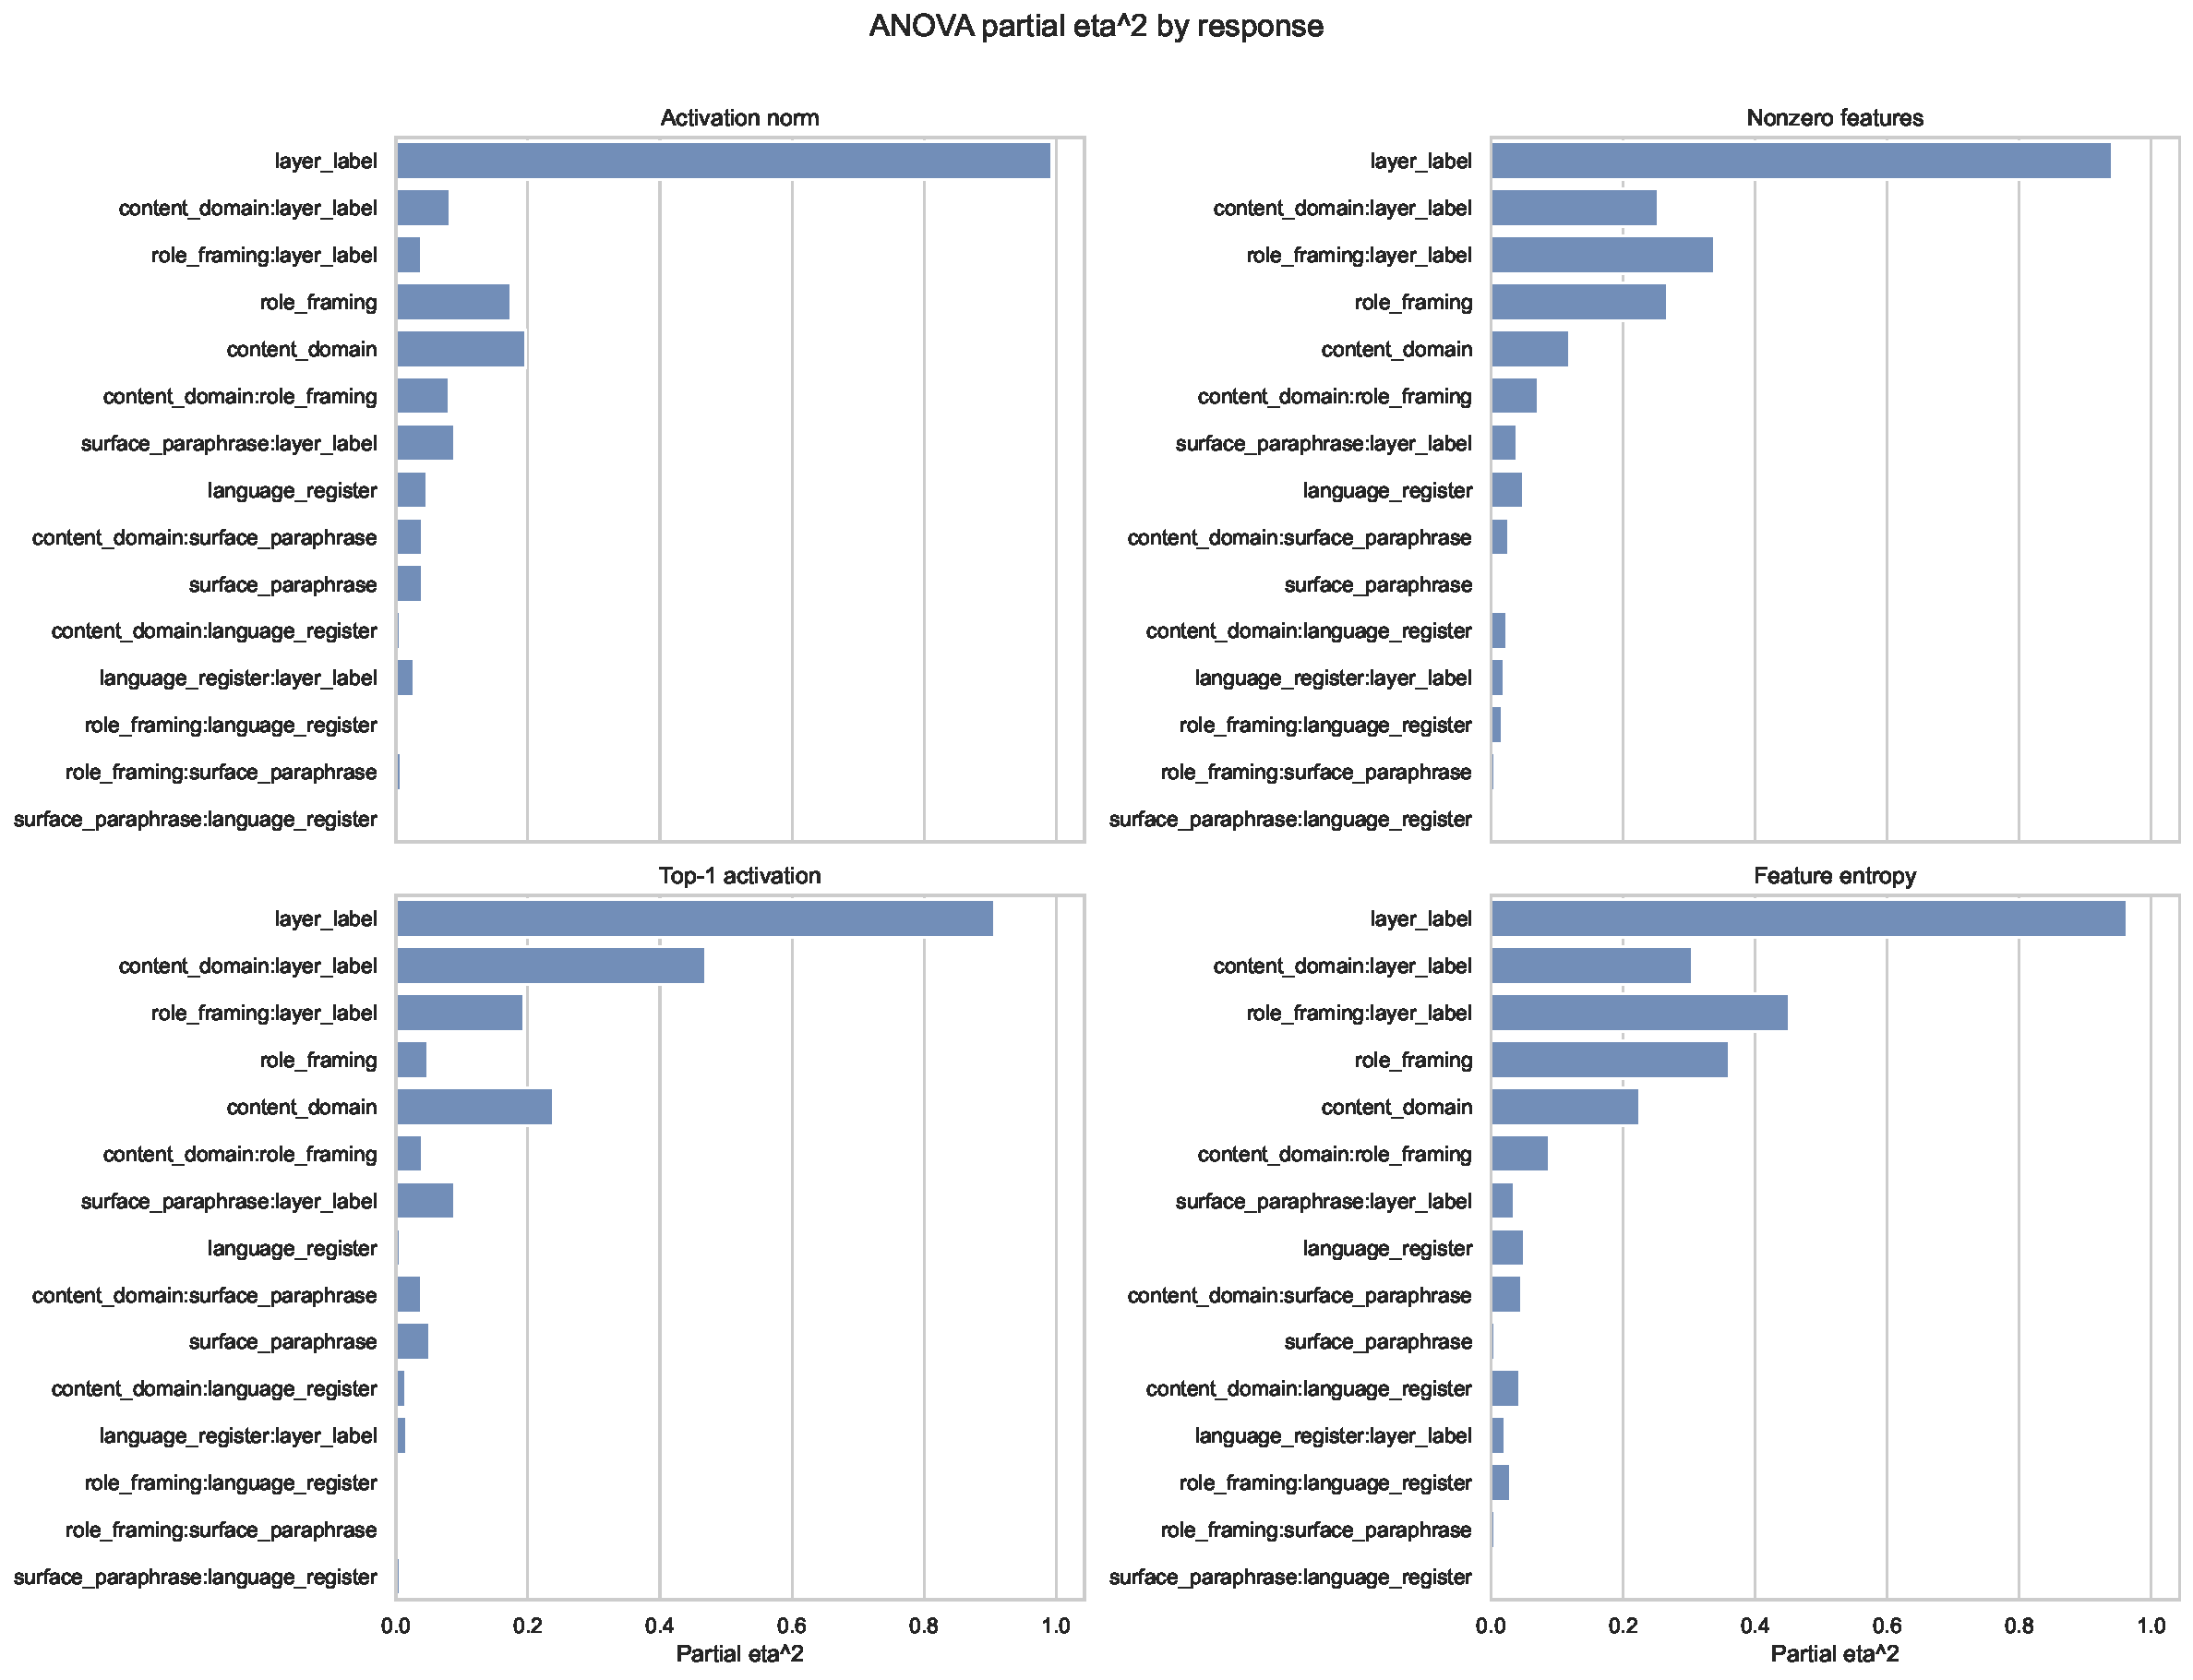
\includegraphics[width=\linewidth]{figures/anova_effect_sizes.pdf}
\caption{Partial $\eta^2$ from five-factor ANOVA models with all main effects and two-way interactions, faceted by response variable.}
\label{fig:anova}
\end{figure}

The three largest terms for each response are:

\begin{center}
\begin{tabular}{llll}
\toprule
Response & Rank 1 & Rank 2 & Rank 3 \\
\midrule
Activation norm & layer (0.993) & content domain (0.197) & role framing (0.175) \\
Nonzero features & layer (0.941) & role framing $\times$ layer (0.338) & role framing (0.267) \\
Top-1 activation & layer (0.907) & content domain $\times$ layer (0.469) & content domain (0.239) \\
Feature entropy & layer (0.963) & role framing $\times$ layer (0.452) & role framing (0.361) \\
\bottomrule
\end{tabular}
\end{center}

\subsection{Variance components}

Figure~\ref{fig:variance} partitions total sum of squares into main effects, summed two-way interactions, summed three-way interactions, and residual. Layer accounts for 98.7\% of total sum of squares in activation norm, 85.8\% in nonzero features, 78.0\% in top-1 activation, and 88.3\% in feature entropy. The non-layer residual and interaction components are largest for top-1 activation.

\begin{figure}[ht]
\centering
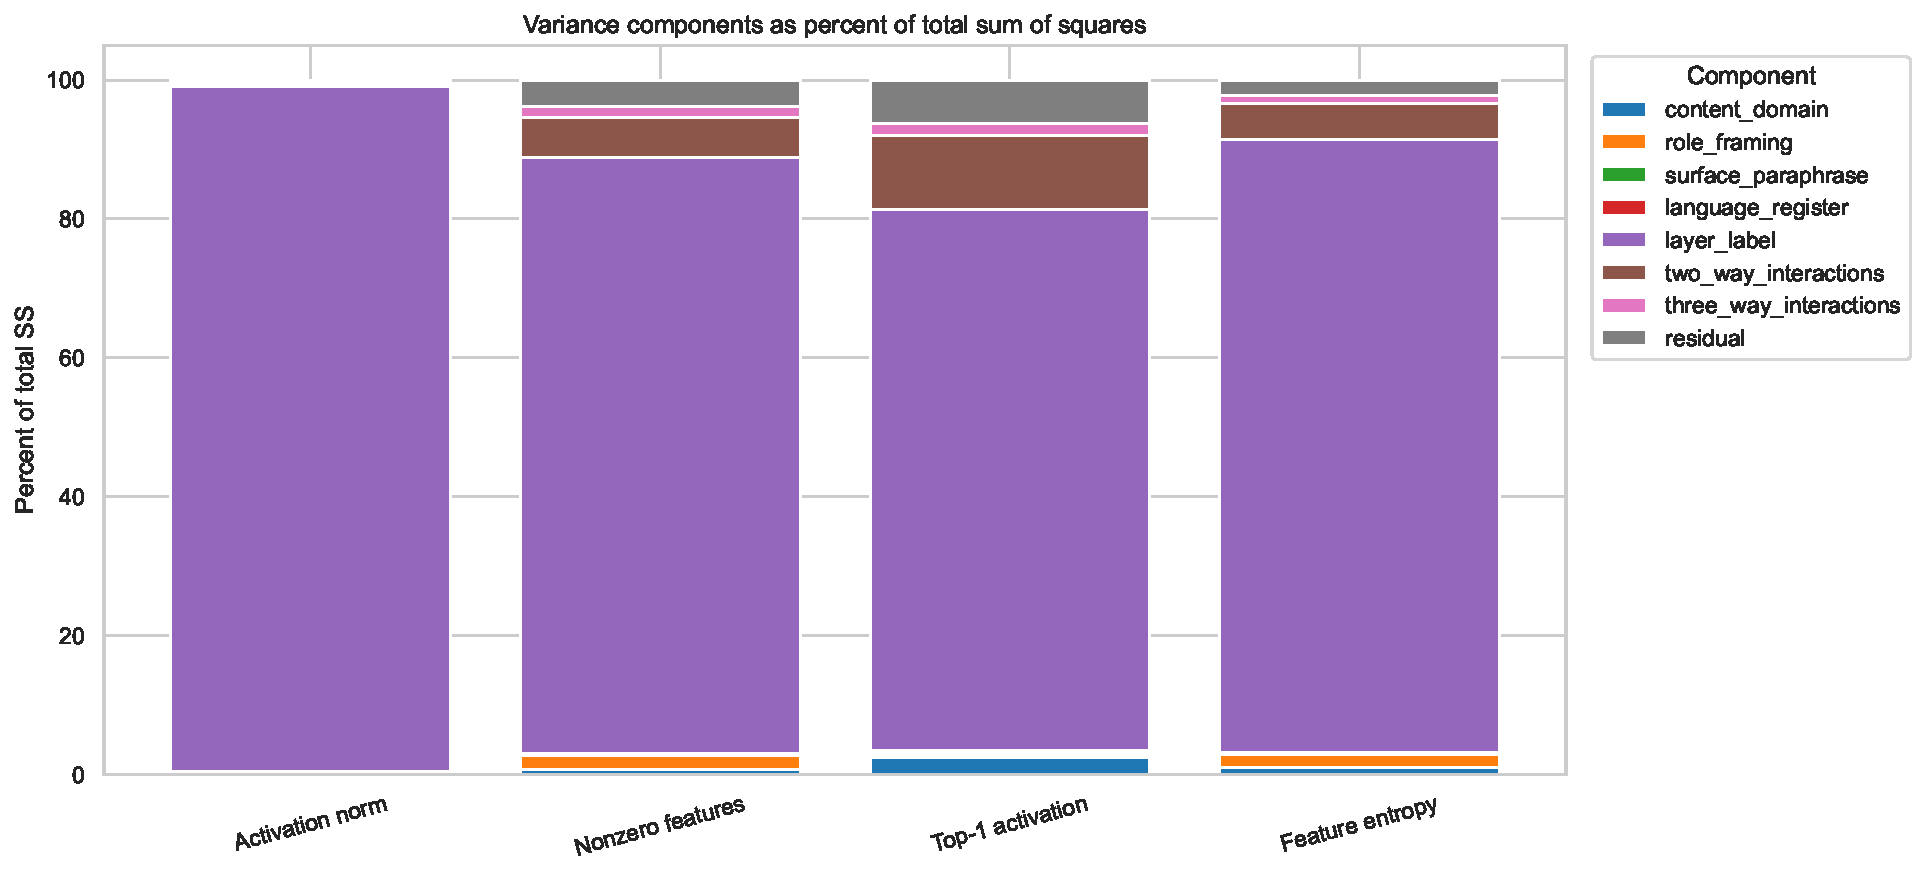
\includegraphics[width=\linewidth]{figures/variance_components_pie.pdf}
\caption{Variance components as percent of total sum of squares. Three-way interactions are summed collectively.}
\label{fig:variance}
\end{figure}

\begin{table}[ht]
\centering
\caption{Variance components as percent of total sum of squares.}
\label{tab:variance}
\begin{tabular}{lrrrrrrrr}
\toprule
Response & Content & Role & Para & Register & Layer & 2-way & 3-way & Residual \\
\midrule
Activation norm & 0.165 & 0.142 & 0.028 & 0.033 & 98.7 & 0.270 & 0.183 & 0.489 \\
Nonzero features & 0.727 & 1.97 & 0.025 & 0.277 & 85.8 & 5.77 & 1.63 & 3.77 \\
Top-1 activation & 2.49 & 0.402 & 0.431 & 0.054 & 78.0 & 10.7 & 1.71 & 6.24 \\
Feature entropy & 0.979 & 1.90 & 0.019 & 0.182 & 88.3 & 5.23 & 1.11 & 2.26 \\
\bottomrule
\end{tabular}
\end{table}

\subsection{Two-way interactions}

Figure~\ref{fig:interactions} summarizes main effects and two-way interactions as symmetric heatmaps. The strongest interactions across all response variables are listed in Table~\ref{tab:strong-interactions}. Interactions with layer are the largest: content-domain-by-layer for top-1 activation, role-framing-by-layer for feature entropy and nonzero features, and content-domain-by-layer for feature entropy and nonzero features.

\begin{figure}[ht]
\centering
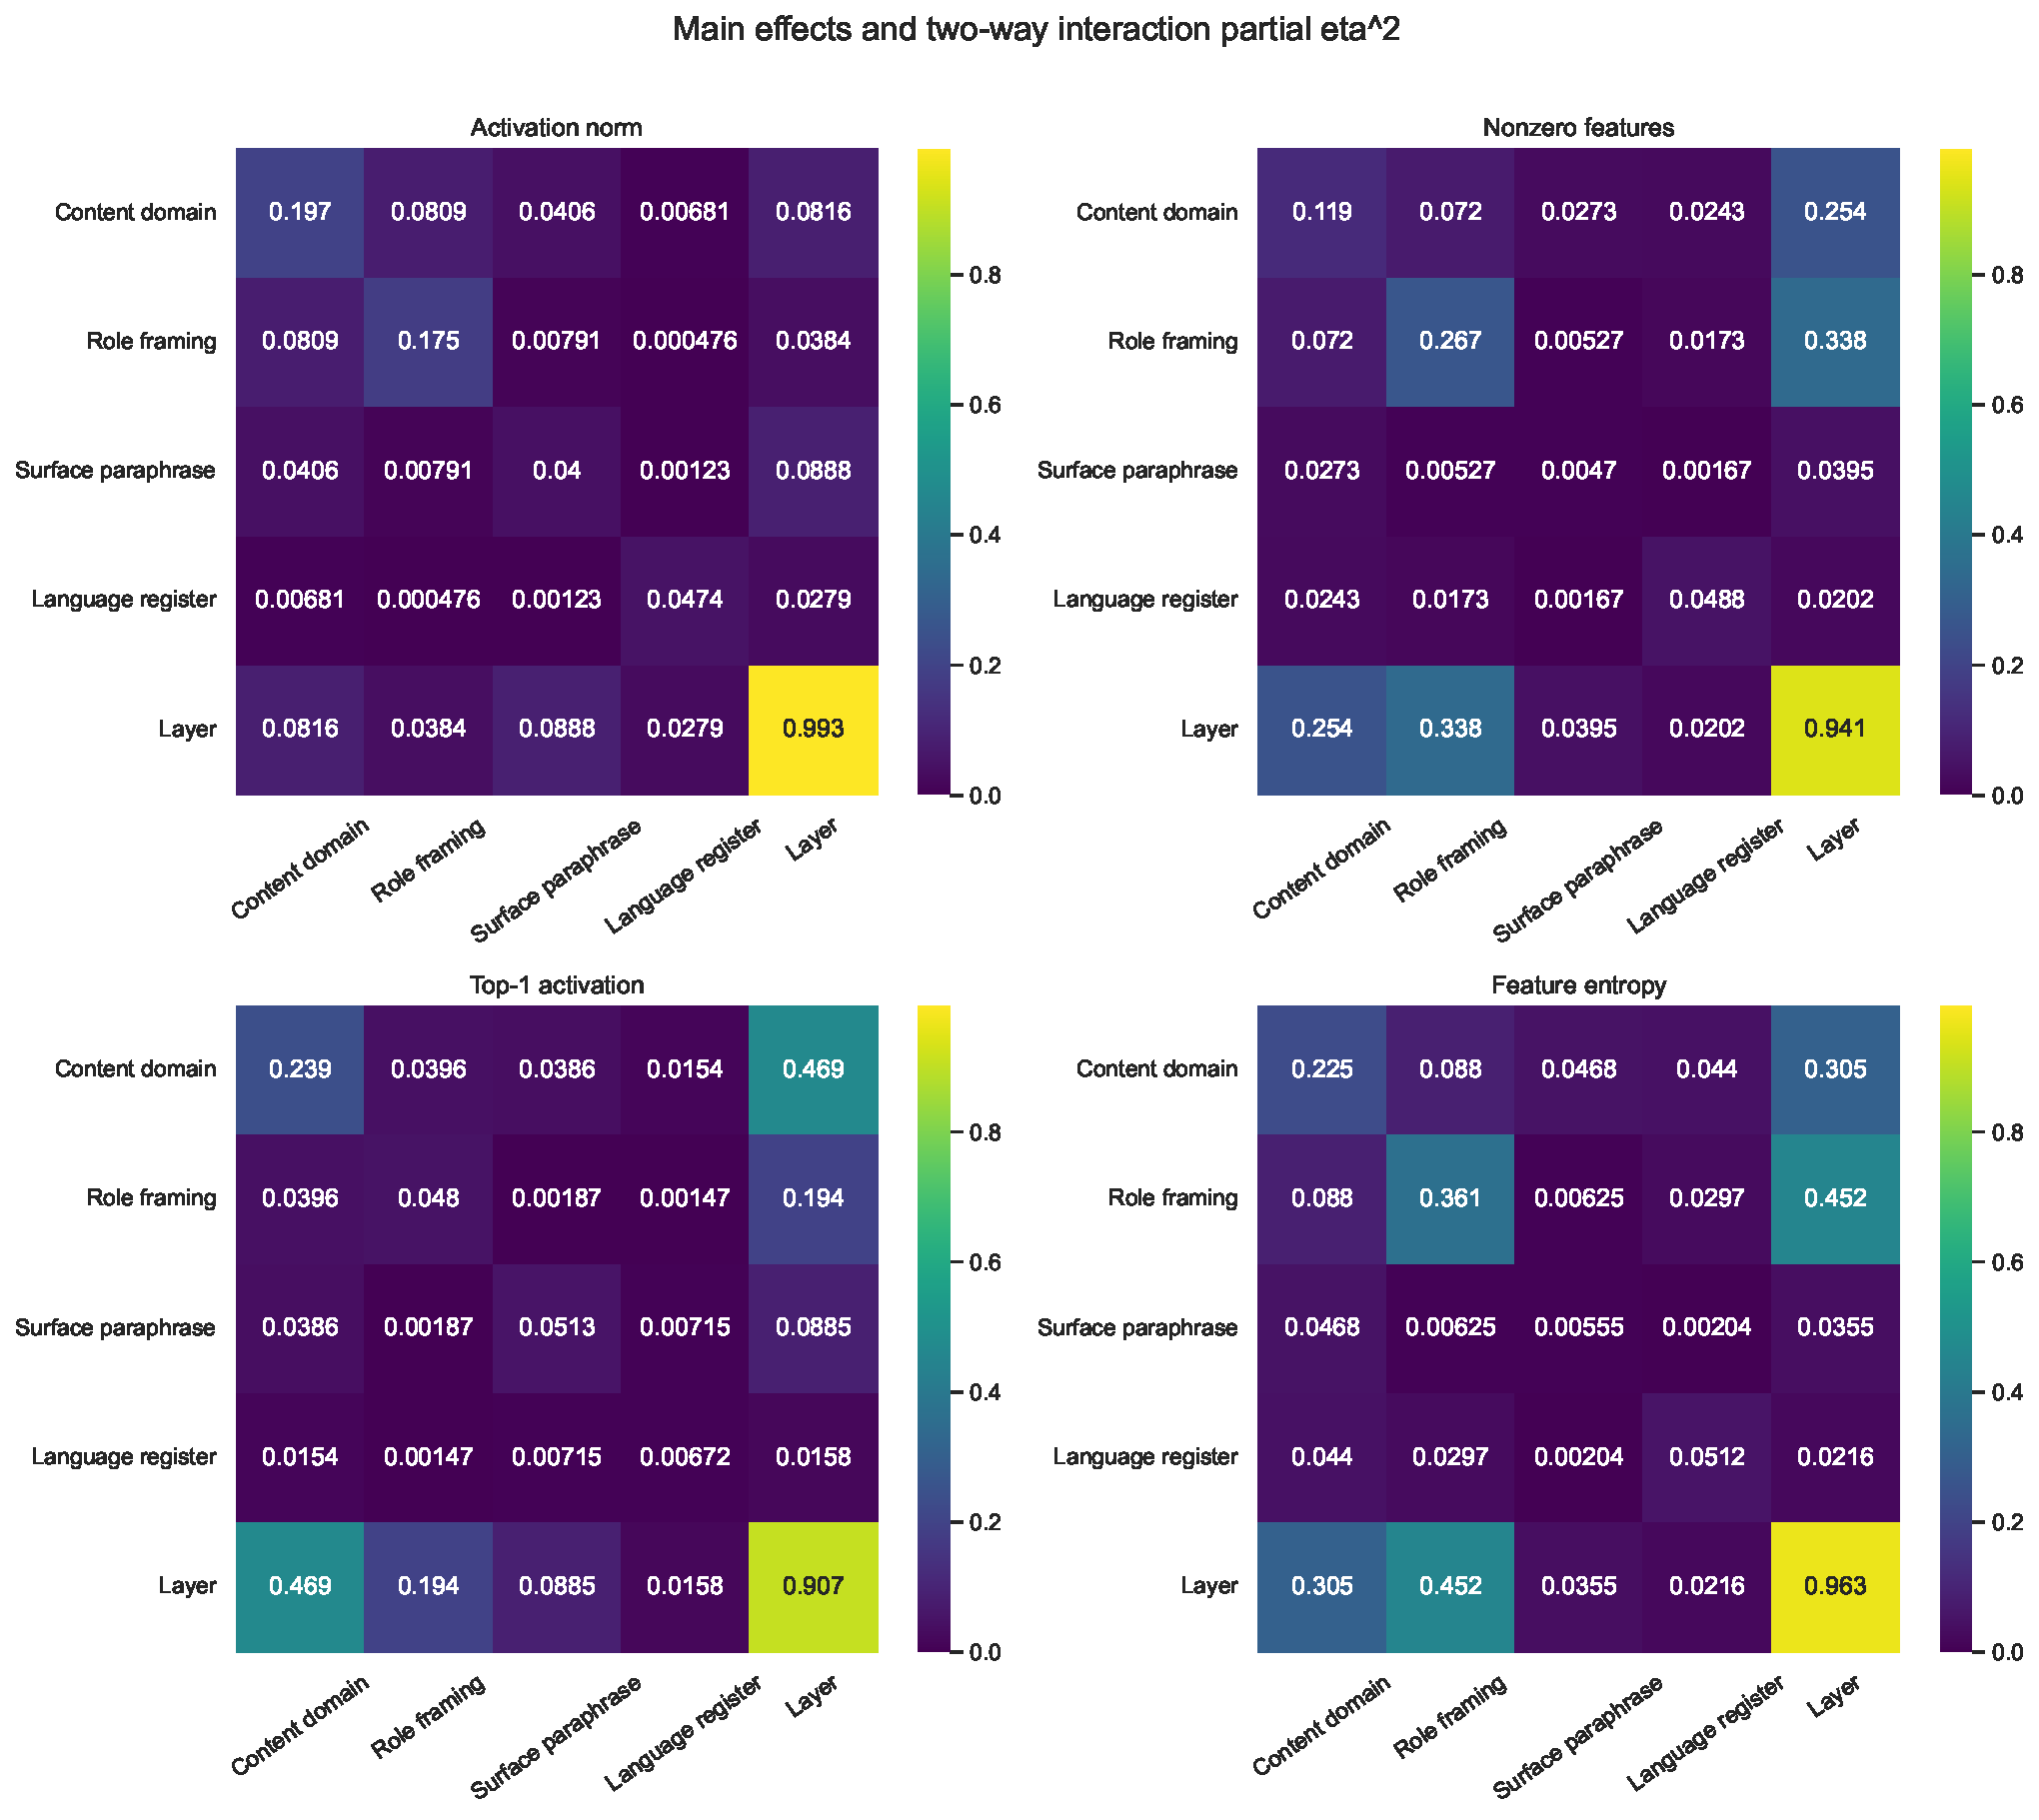
\includegraphics[width=\linewidth]{figures/interaction_heatmap.pdf}
\caption{Main-effect and two-way interaction partial $\eta^2$ values for the four scalar response variables. Diagonal cells show main effects; off-diagonal cells show two-way interactions.}
\label{fig:interactions}
\end{figure}

\begin{table}[ht]
\centering
\caption{Five strongest two-way interactions across response variables.}
\label{tab:strong-interactions}
\begin{tabular}{lll}
\toprule
Response & Interaction & Partial $\eta^2$ \\
\midrule
Top-1 activation & content domain $\times$ layer & 0.469 \\
Feature entropy & role framing $\times$ layer & 0.452 \\
Nonzero features & role framing $\times$ layer & 0.338 \\
Feature entropy & content domain $\times$ layer & 0.305 \\
Nonzero features & content domain $\times$ layer & 0.254 \\
\bottomrule
\end{tabular}
\end{table}

\subsection{Full-spectrum similarity and block structure}

Scalar ANOVA compresses each cell to one response. To retain more feature geometry, the analysis also considers full 16,384-dimensional SAE encodings. Figure~\ref{fig:block} shows a permutation test for role-framing block diagonality on the 27 factual-recall \texttt{fr1} layer-12 cells. The observed statistic is the mean within-block cosine similarity minus mean between-block cosine similarity. Role framing has observed statistic 0.0912; among 1000 random label shuffles, no null draw matched or exceeded the observed statistic, so we report $p < 0.001$ for this finite permutation run. Surface paraphrase and language register do not show comparable evidence of block structure in this focal matrix.

\begin{figure}[ht]
\centering
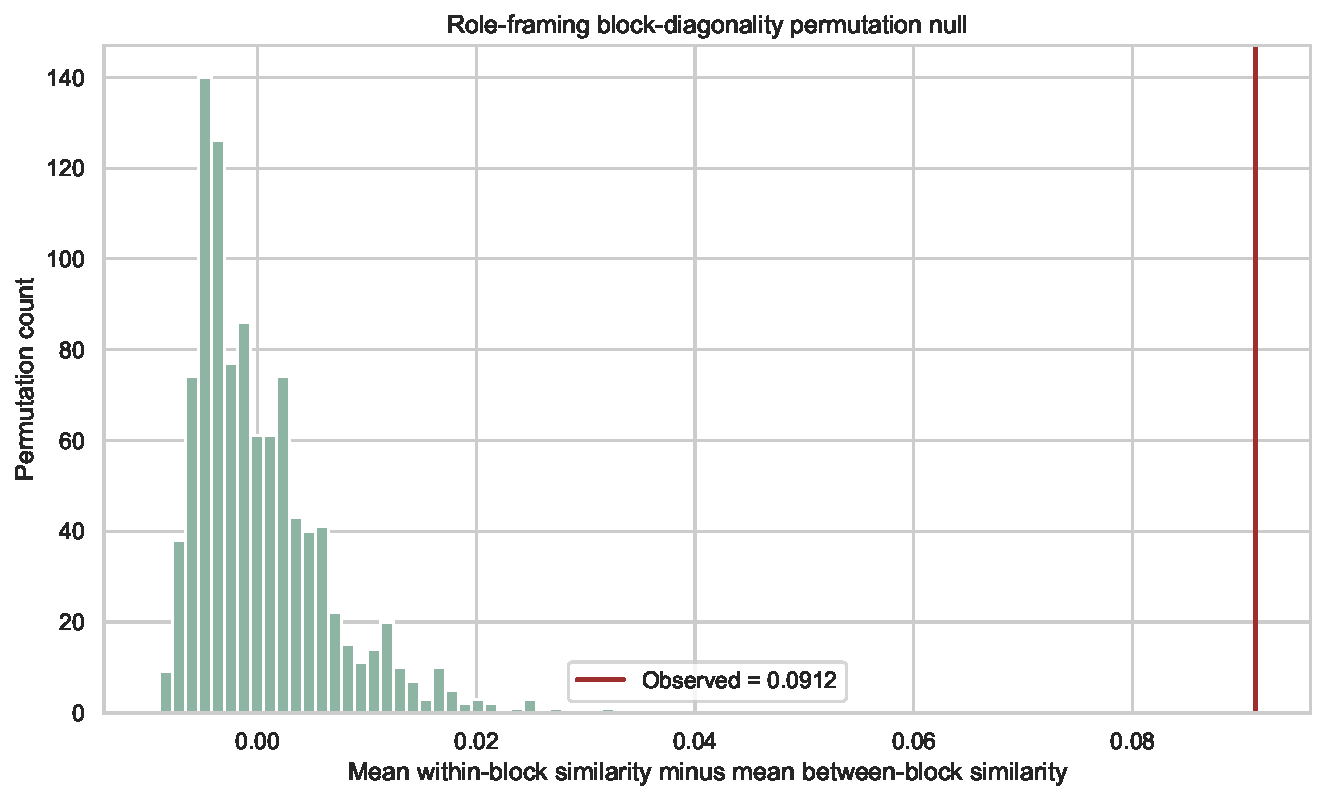
\includegraphics[width=0.85\linewidth]{figures/block_diagonality_permutation.pdf}
\caption{Permutation null distribution for role-framing block diagonality in the factual-recall \texttt{fr1} layer-12 full-spectrum cosine matrix. The red line marks the observed within-minus-between statistic.}
\label{fig:block}
\end{figure}

\begin{table}[ht]
\centering
\caption{Block-diagonality permutation tests for the 27 factual-recall \texttt{fr1} layer-12 cells.}
\label{tab:block}
\begin{tabular}{lrrrr}
\toprule
Block factor & Observed & Mean within & Mean between & Empirical $p$ \\
\midrule
Role framing & 0.0912 & 0.959 & 0.868 & $<0.001$ \\
Surface paraphrase & -0.00394 & 0.893 & 0.897 & 0.685 \\
Language register & 0.00247 & 0.897 & 0.895 & 0.279 \\
\bottomrule
\end{tabular}
\end{table}

\subsection{Retrospective Latin-style subsampling}

The full design contains 81 prompt-side cells and five content-ID replicates per domain. To ask whether a reduced design could have recovered the main-factor ranking, we constructed categorical Latin-style subsamples at $K=27$, $K=18$, and $K=9$ prompt cells, then included all three layers for selected prompt cells. The $K=27$ design uses a $3^3$ Latin-style construction over content domain, role framing, and surface paraphrase, assigning language register by modular cycling. The random seed is 42.

Figure~\ref{fig:lhs} compares main-effect partial $\eta^2$ values from the full factorial design to these subsamples. At $K=27$, the Spearman rank correlation between full and subsampled main-effect rankings is 0.9 for all four responses. At $K=18$, recovery weakens substantially. At $K=9$, the subsample can become actively misleading: the ranking correlation is negative for nonzero features ($-0.9$) and top-1 activation ($-0.6$), indicating that very small Latin-style subsamples can invert the apparent factor ordering rather than merely add noise.

\begin{figure}[ht]
\centering
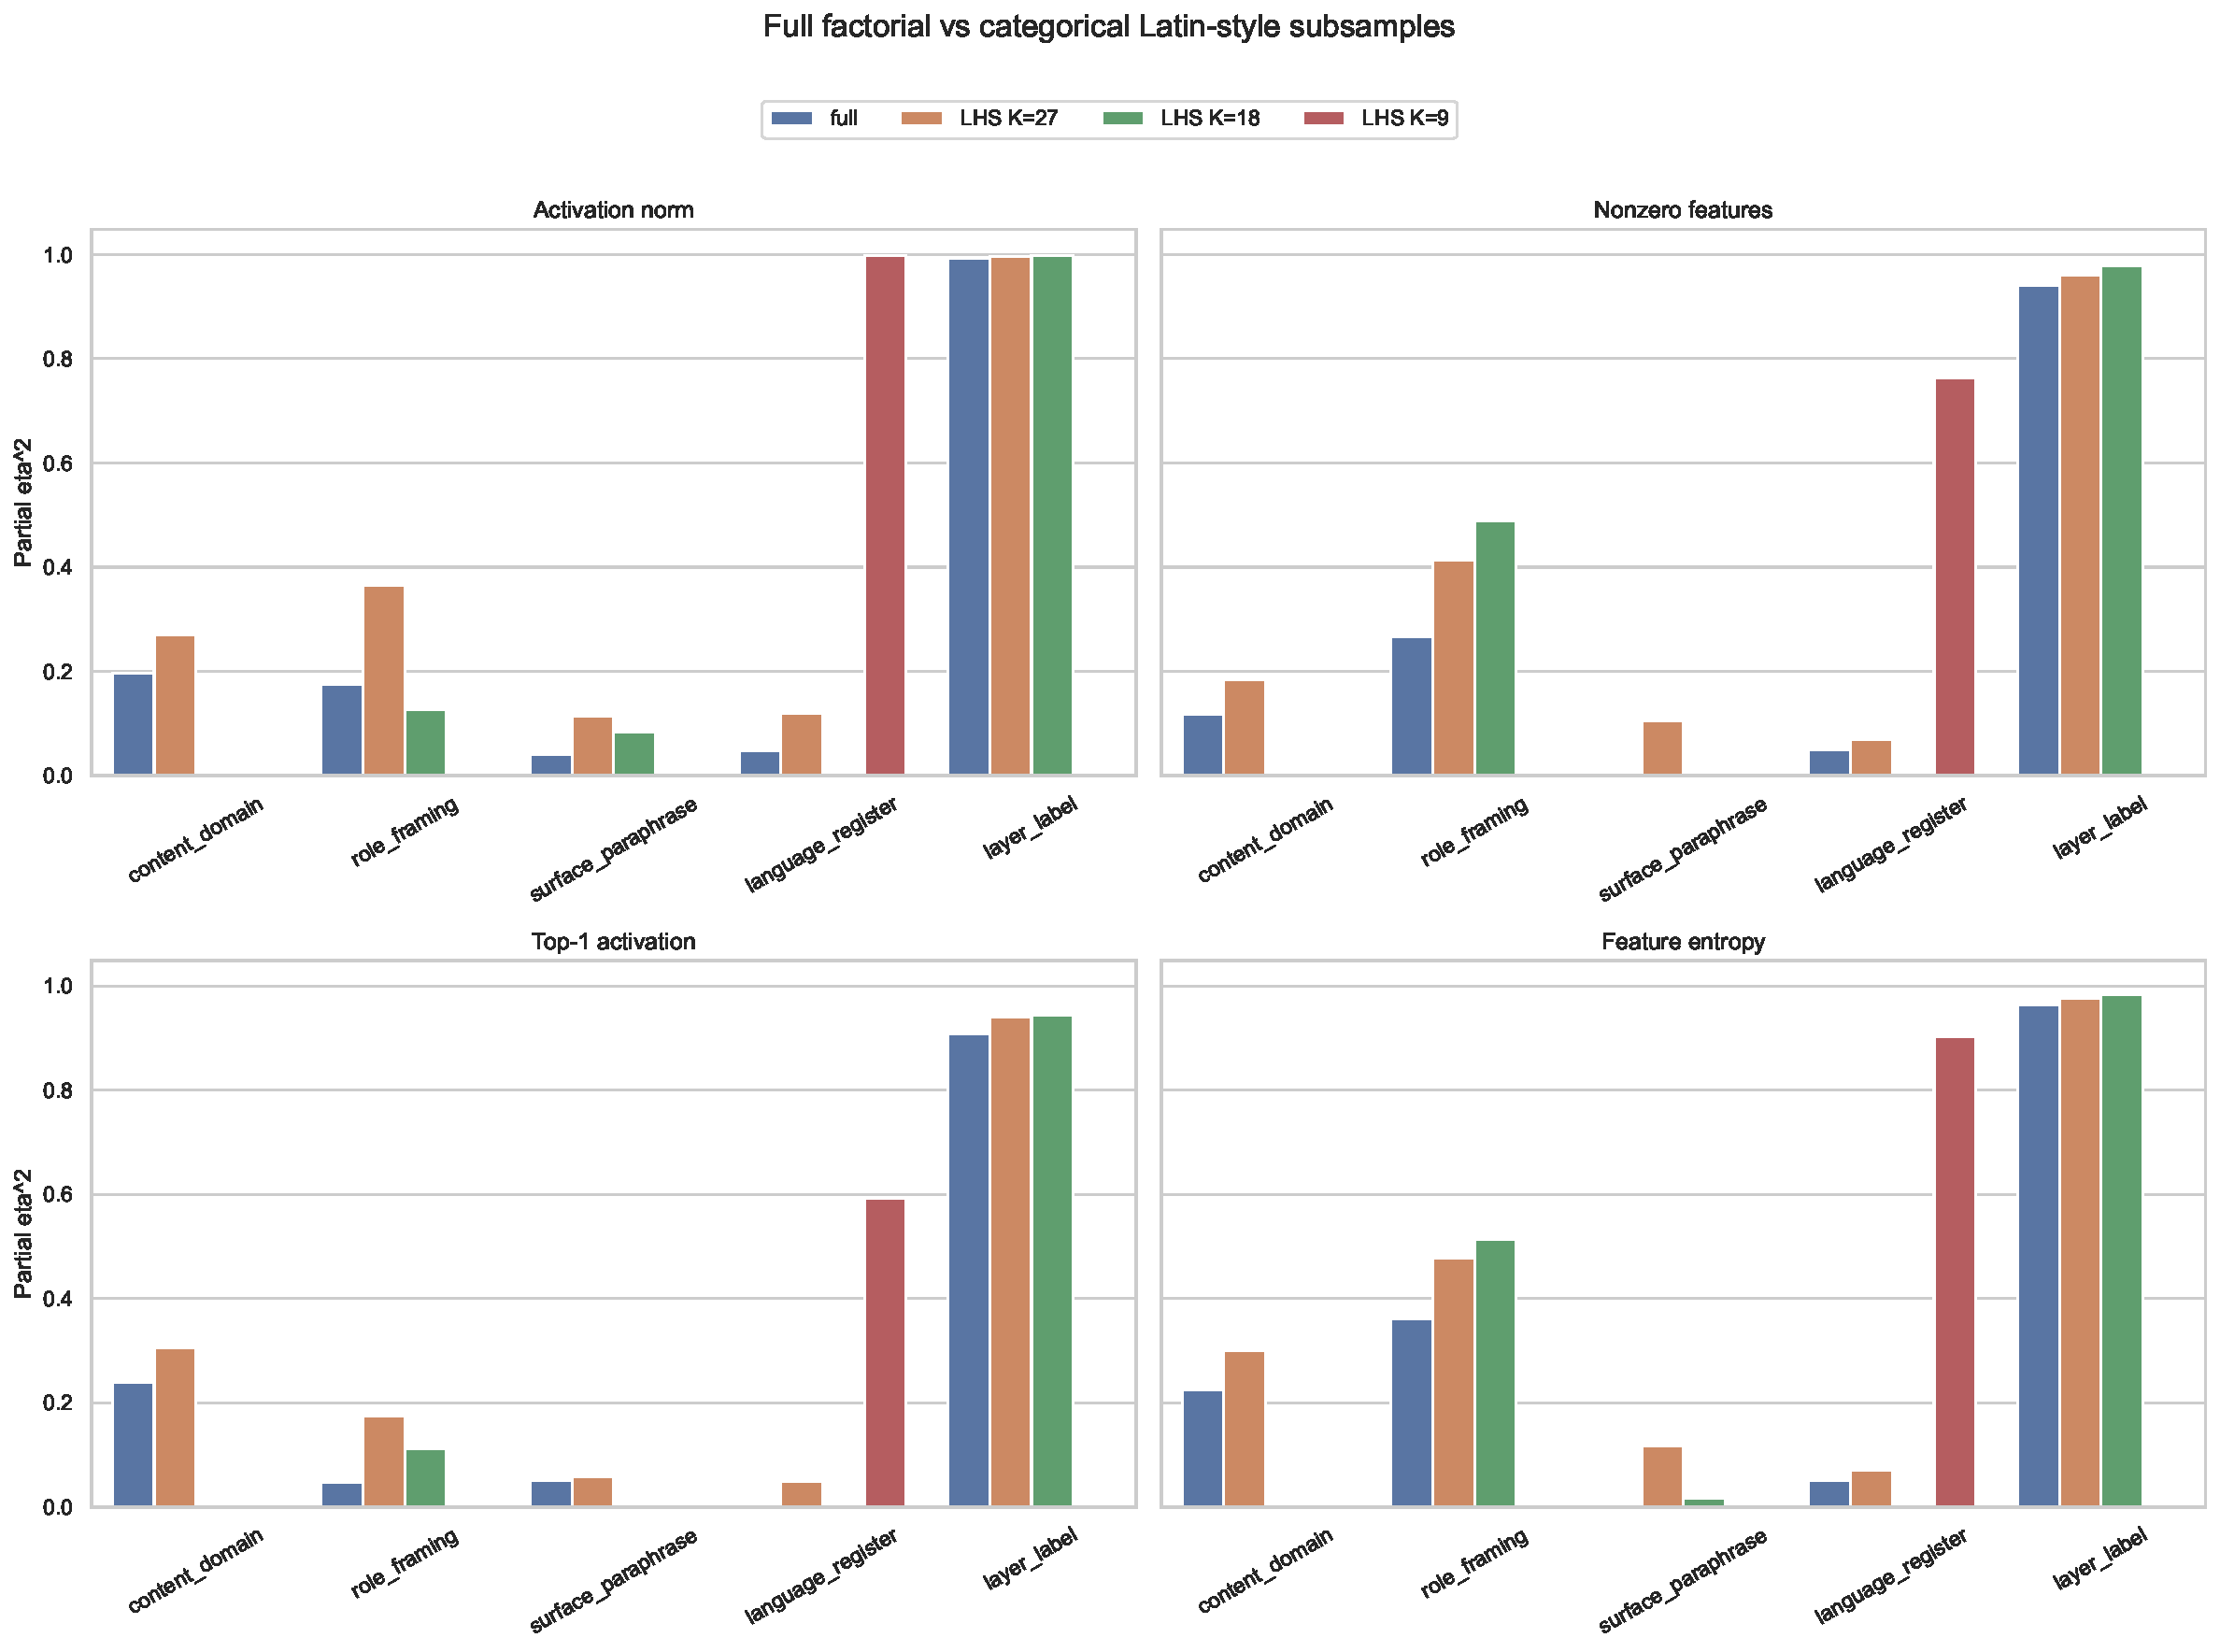
\includegraphics[width=\linewidth]{figures/lhs_vs_full_comparison.pdf}
\caption{Main-effect partial $\eta^2$ under the full factorial design and three categorical Latin-style subsamples.}
\label{fig:lhs}
\end{figure}

\begin{table}[ht]
\centering
\caption{Spearman correlation between full-factorial and subsampled main-effect rankings.}
\label{tab:lhs}
\begin{tabular}{lrrr}
\toprule
Response & $K=27$ & $K=18$ & $K=9$ \\
\midrule
Activation norm & 0.9 & 0.5 & 0.0 \\
Nonzero features & 0.9 & 0.6 & -0.9 \\
Top-1 activation & 0.9 & 0.3 & -0.6 \\
Feature entropy & 0.9 & 0.6 & 0.3 \\
\bottomrule
\end{tabular}
\end{table}

\section{Discussion}

The most stable high-level result is that layer dominates the scalar SAE-response variables, though layer here is confounded with SAE identity and should not be read as a pure depth claim. This is not surprising, because residual-stream scale, SAE dictionary, and representation geometry all change across layer. However, the interaction terms show that layer is not merely an additive offset. Content domain and role framing change response variables differently depending on the layer, especially for top-1 activation, feature entropy, and nonzero feature count.

These interaction effects have a methodological implication for mechanistic-interpretability practice. Reports that present SAE measurements at a single layer cannot distinguish layer-specific patterns from model-general ones; the same prompt factor may have different apparent effects on SAE features at different depths. Likewise, studies that vary content while holding role framing fixed, or vary role framing while holding content fixed, will under-report the variance attributable to the factors held constant and cannot estimate their interactions. The value of the factorial design is therefore not only that it gives cleaner estimates, but that it makes such interaction structure visible at all.

The block-diagonality result is narrower but more geometrically direct. In the focal factual-recall \texttt{fr1} layer-12 set, role framing organizes full-spectrum SAE cosine similarities into detectable blocks. This remains true after shuffling the 27 cell labels while preserving 9/9/9 block sizes. By contrast, paraphrase and register do not produce comparable block structure in that same matrix. This suggests that, at least for this focal item and layer, conversational form has a stronger geometric footprint than local wording or register.

The retrospective subsampling result gives a practical design hint. A 27-cell categorical Latin-style design recovers the full-factorial main-effect ranking well in this run, but smaller designs are not merely less precise: at $K=9$, two response variables show inverted main-effect rankings relative to the full design. This does not establish a general sampling theorem. It does suggest that reduced designs may be useful for exploratory sweeps only when followed by full-factorial confirmation on the factors that appear promising.

\section{Limitations}

First, this report analyzes only one model family, one model size, and three layers. Second, the layer factor confounds transformer depth with SAE dictionary identity; the result that layer dominates is a real measurement result, but it should not be read as a pure depth effect independent of the SAE used at each layer. Third, the response variables are scalar summaries of sparse encodings. They are useful for factorial decomposition, but they discard much of the feature geometry. Fourth, no SAE feature is interpreted semantically here. The report deliberately avoids Neuronpedia lookup or causal feature intervention. Finally, the corpus is controlled but small; five content IDs per domain are enough for this measurement study, not for broad claims about all prompts or all semantic domains.

\section{Conclusion}

This experiment shows that a small fully crossed prompt design can be combined with open Gemma Scope SAEs to produce analyzable, persisted measurements of SAE feature stability. The resulting dataset supports classical factorial decomposition, full-spectrum similarity checks, block-diagonality tests, and retrospective reduced-design comparisons. The strongest pattern is layer dominance, followed by layer interactions with content domain and role framing. In a focal layer-12 similarity matrix, role framing produces a quantitatively detectable block structure, while paraphrase and register do not. These results provide a concrete measurement basis for deciding which prompt factors and layers deserve more focused follow-up.

\appendix

\section{Supplementary Figures}

\begin{figure}[ht]
\centering
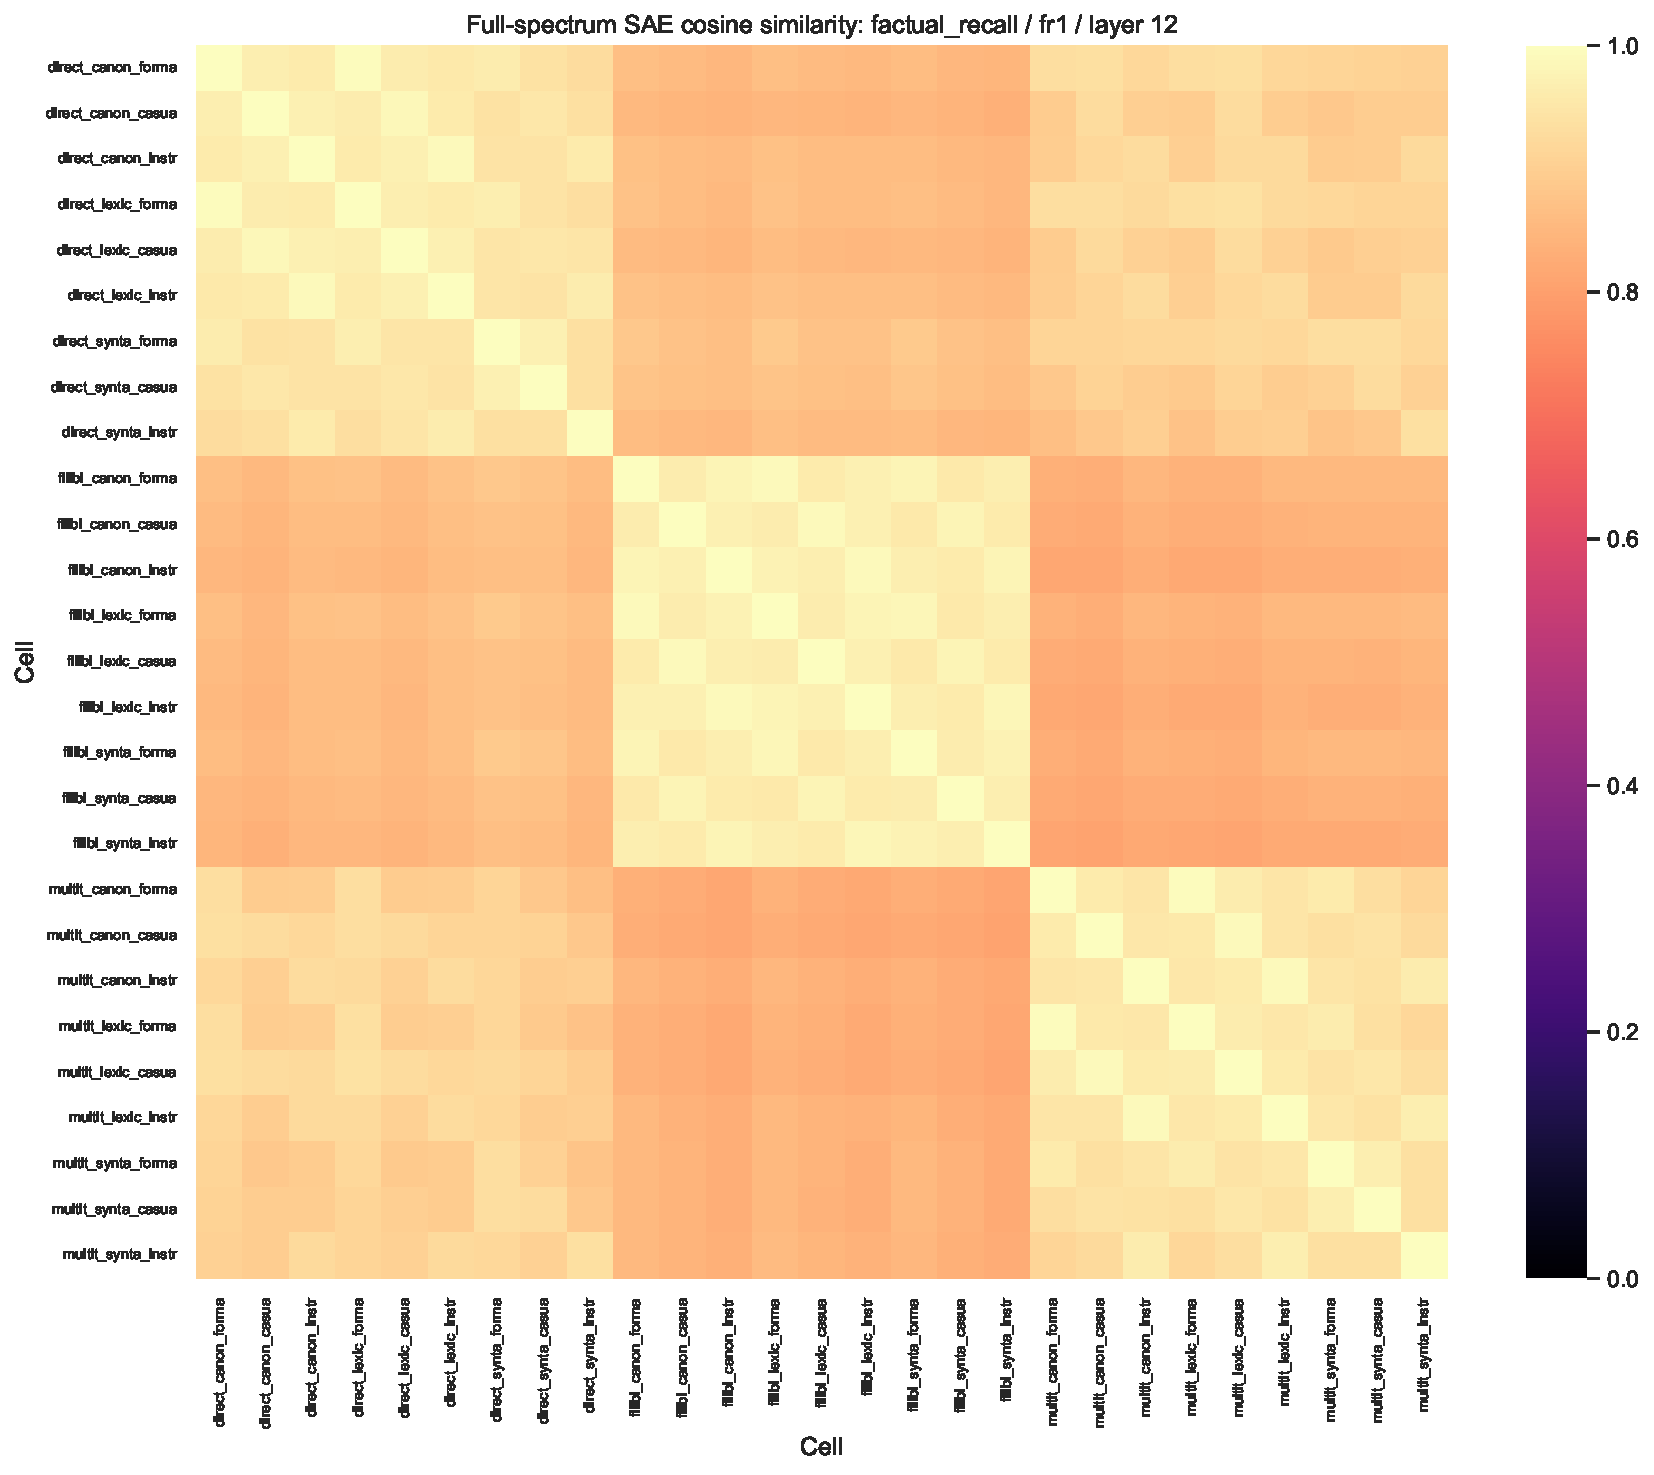
\includegraphics[width=\linewidth]{figures/full_spectrum_overlap_heatmap.pdf}
\caption{Full-spectrum SAE cosine similarity for the 27 factual-recall \texttt{fr1} layer-12 cells.}
\label{fig:full-spectrum}
\end{figure}

\begin{figure}[ht]
\centering
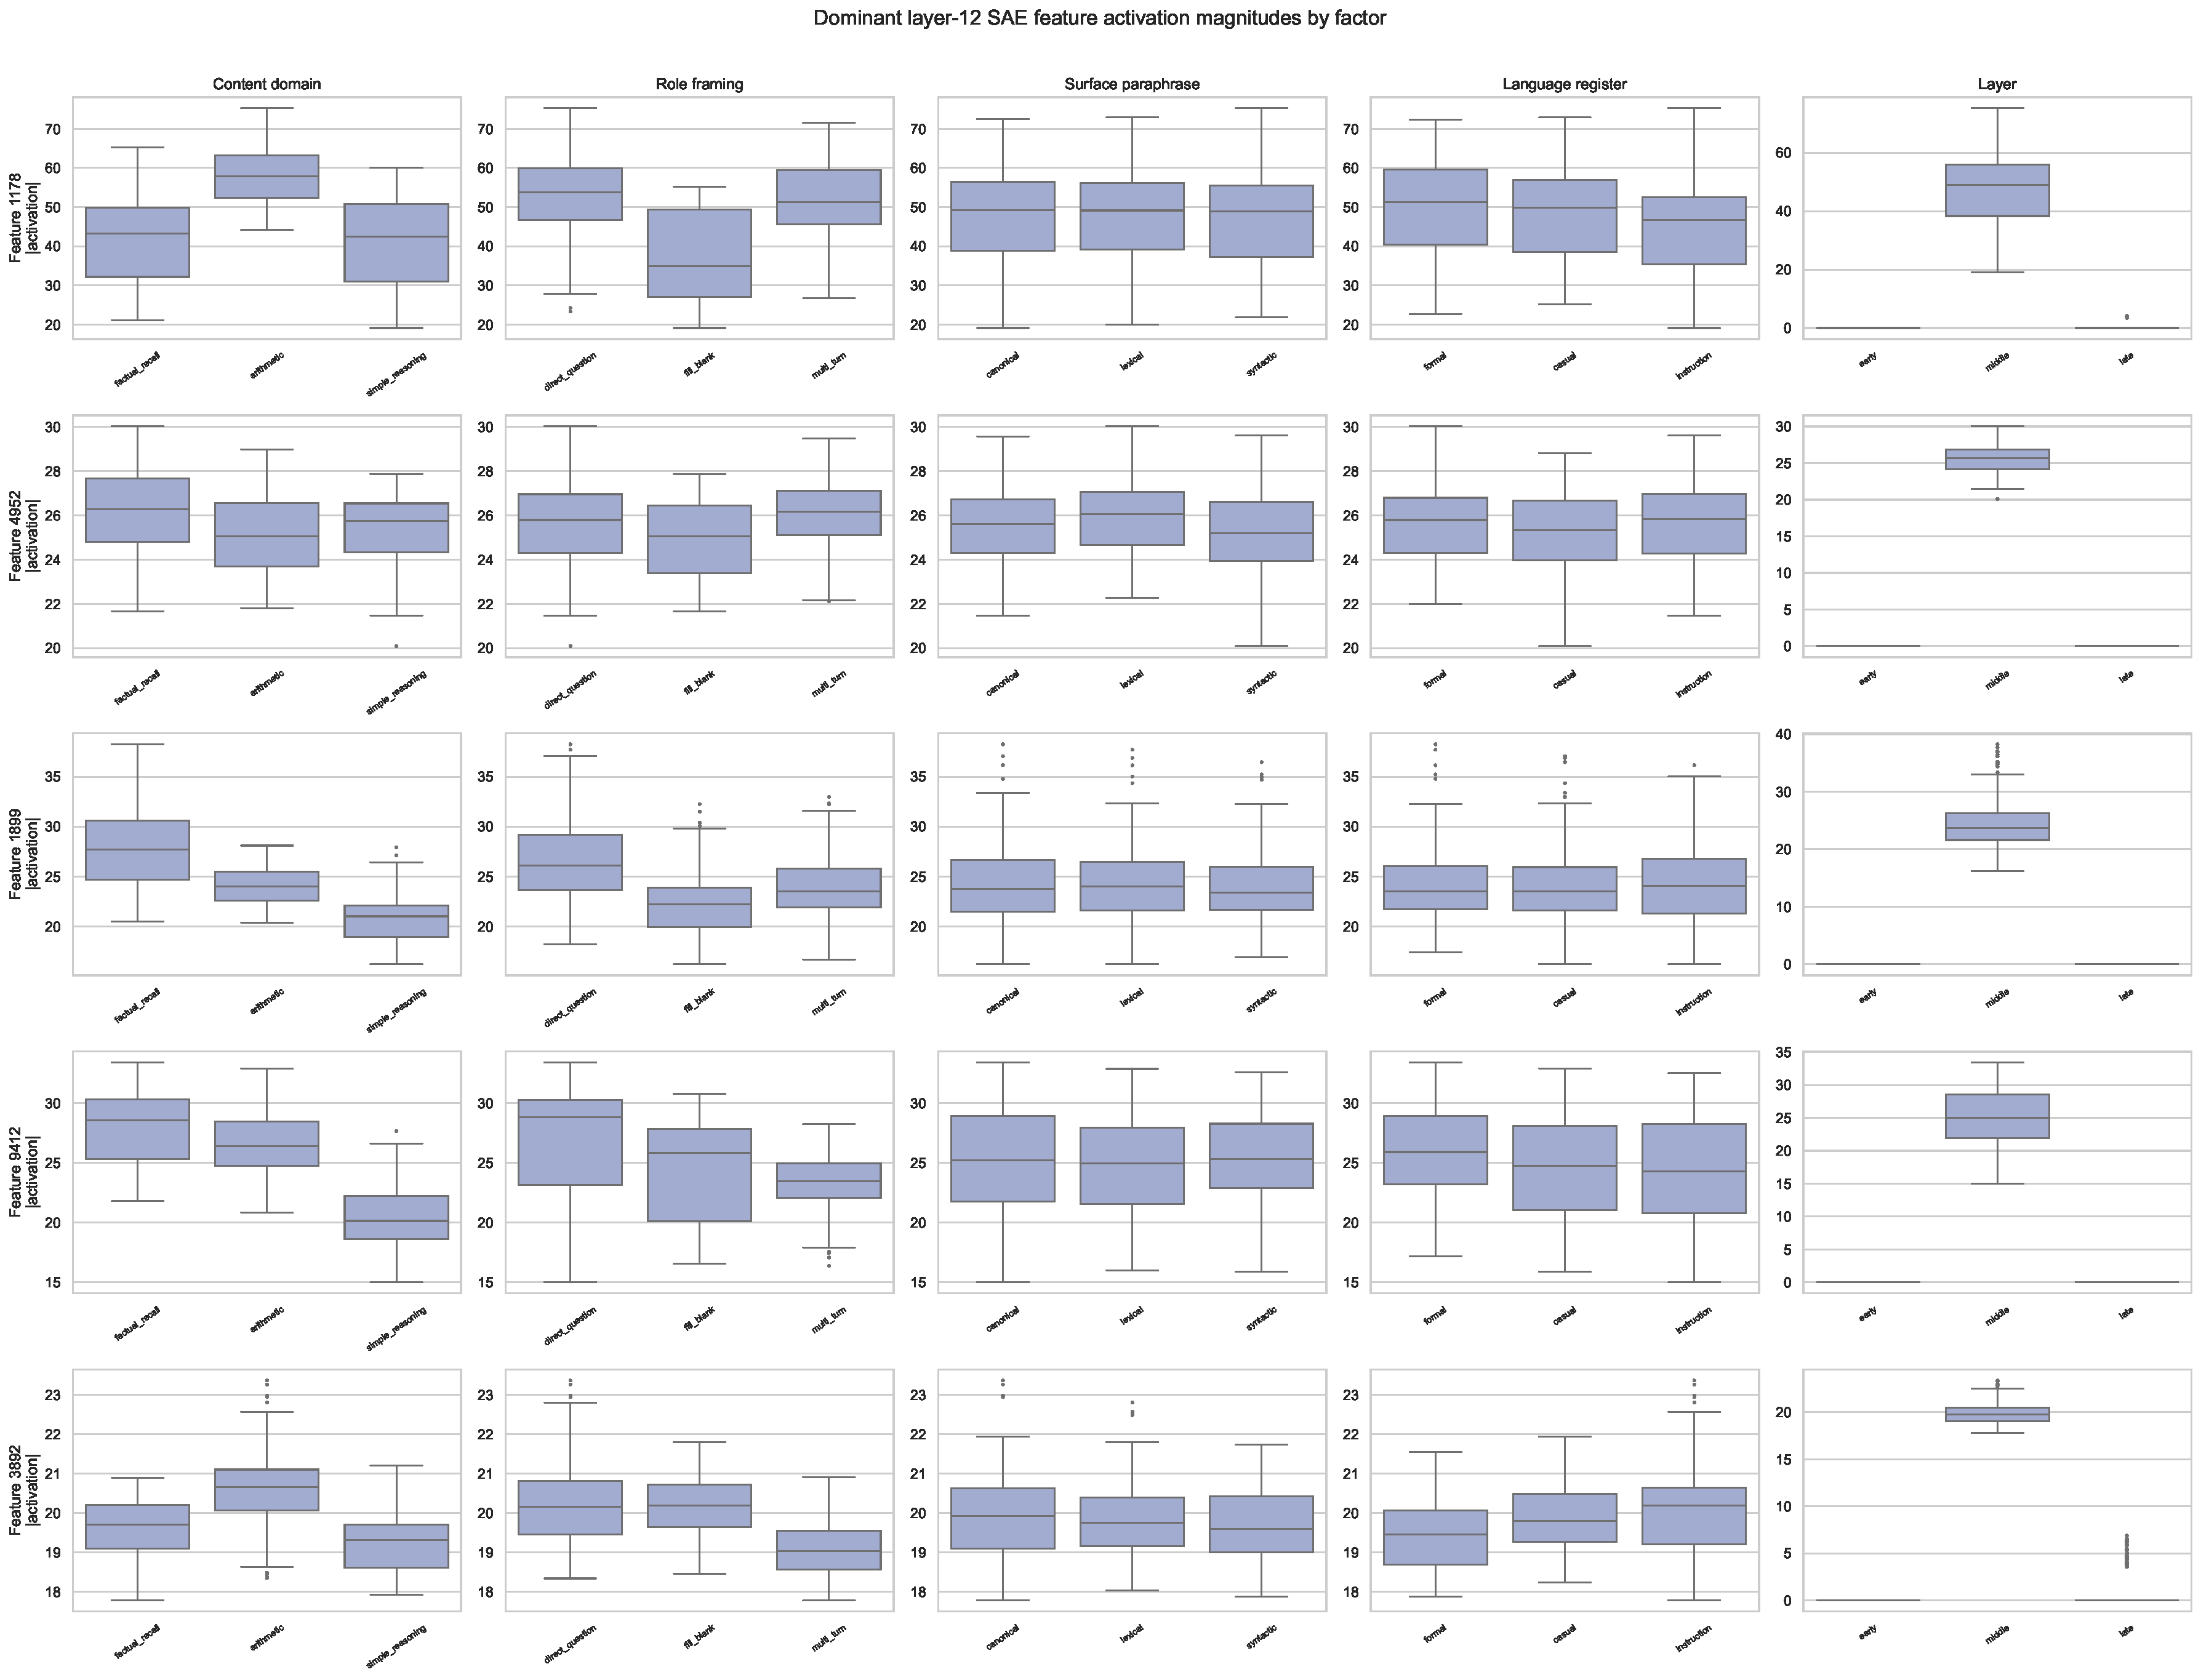
\includegraphics[width=\linewidth]{figures/dominant_feature_variation.pdf}
\caption{Variation in the five most frequently top-ranked layer-12 SAE features across factors.}
\label{fig:dominant}
\end{figure}

\bibliographystyle{plainnat}
\bibliography{references}

\end{document}
